\section{Introduction}

Document-level relation extraction (DocRE) requires identifying semantic relations between entity pairs across multiple sentences, a task where encoder-based methods such as \citet{zhou2021atlop} long dominated.
Recent LLM-based approaches have closed this gap: \citet{autore2024} fine-tune LLMs with structured decomposition, \citet{xu2024lmrc} frame it as multi-choice reading comprehension, and \citet{xu2025docksrag} combine retrieval-augmented generation with structured knowledge.
These methods approach or surpass encoder baselines on DocRED \citep{yao2019docred} and Re-DocRED \citep{tan2022redocred} in extraction accuracy, yet every one outputs bare relation triplets $(e_h, r, e_t)$ without indicating \emph{which sentences} support each prediction.
Without evidence, a clinician reviewing a ten-page case report must manually locate the sentences that support each extracted drug interaction, a bottleneck that undermines trust in automated extraction.

\begin{figure*}[!t]
\centering
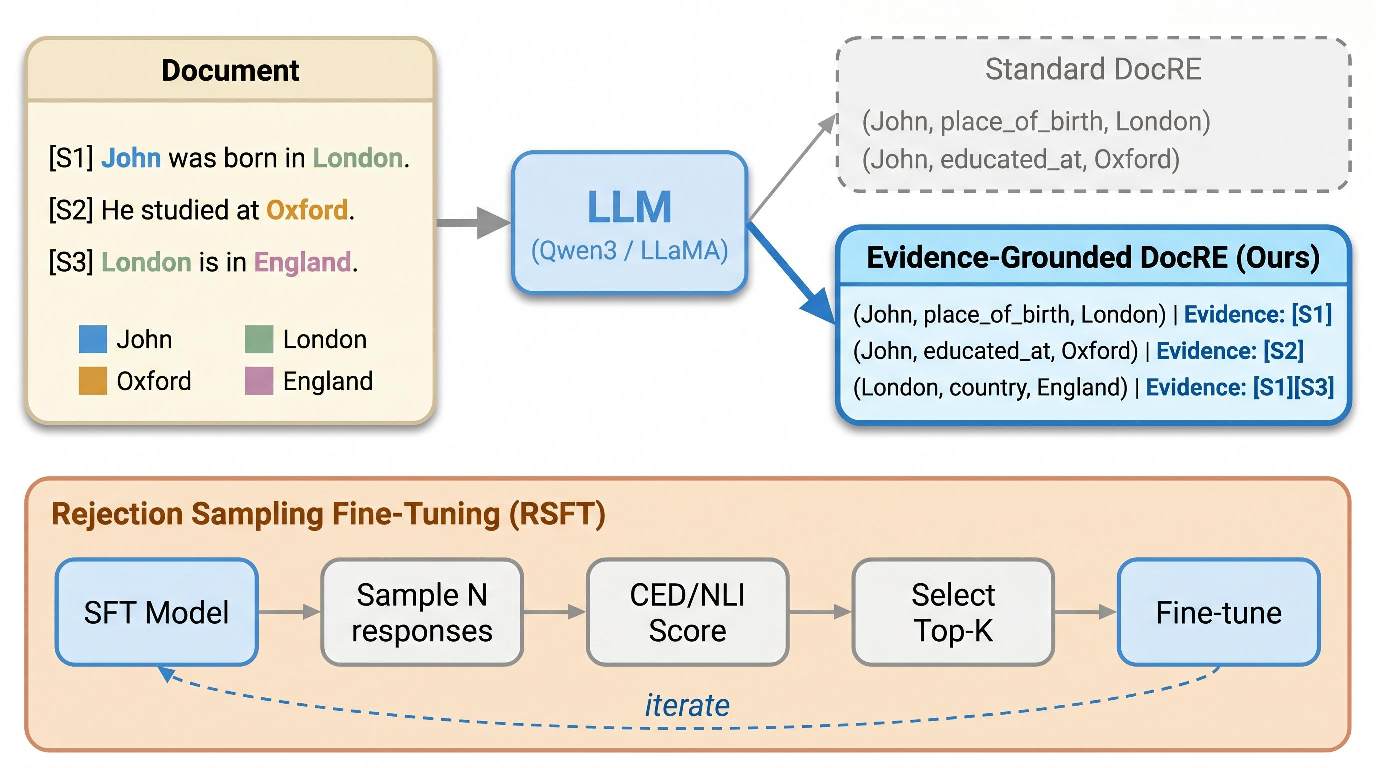
\includegraphics[width=0.92\textwidth]{fig_overview.pdf}
\vspace{-2mm}
\caption{Evidence-grounded DocRE produces relation triples with supporting sentence indices, unlike standard DocRE which outputs bare triples. RSFT selects the top-$k$ of $N$ candidates per document, scored by Contrastive Evidence Discrimination (CED; \S\ref{sec:ced}), for fine-tuning.}
\label{fig:overview}
\end{figure*}

Encoder-based methods have partially addressed this need: \citet{xiao2022sais} introduce sentence-level evidence supervision as an auxiliary signal, and \citet{ma2023dreeam} extend this with dynamic evidence retrieval through memory attention.
Both produce evidence and improve extraction, but encoder methods now trail LLM-based approaches in accuracy.
The community faces a gap: the most accurate extractors provide no evidence, while evidence-capable methods are no longer competitive.

This gap reflects a structural difference.
In encoder methods, evidence retrieval is classification that regularizes the encoder at negligible cost; in LLM-based DocRE, evidence requires the model to \emph{generate} additional output tokens per triple, increasing output length and decoding complexity.
The na\"{i}ve expectation is that this generation cost always harms extraction accuracy.
Our experiments show this expectation is wrong.
The evidence tax---the accuracy cost of jointly generating evidence---is not a fixed penalty but a landscape shaped by model capacity, optimization paradigm, and training data quality.
Within the Qwen3 family, evidence generation \emph{benefits} extraction at 1.7B ($-$5.63pp Ign-F1, partly through halving output duplication) but is approximately neutral at $\geq$4B (+0.25$\pm$0.47pp at 4B).
Gradient-based optimization amplifies this competition, as GRPO collapses extraction under constrained precision and DPO progressively trades extraction for evidence, while discrete sample selection (RSFT) avoids the trade-off entirely by filtering outputs rather than pushing gradients. To quantify this decoupling, we define the Evidence-Decoupling Ratio (EDCR), a diagnostic metric that measures the fraction of cited evidence not supported by gold annotations.

We study evidence-grounded DocRE as a structured generation task and compare three post-training paradigms across three fully evaluated scales (1.7B, 4B, 8B) with 14B validation, two model families, and two datasets: Group Relative Policy Optimization (GRPO) \citep{shao2024deepseekmath}, Direct Preference Optimization (DPO) \citep{rafailov2023direct}, and Rejection Sampling Fine-Tuning (RSFT), building on Self-Taught Reasoner (STaR) \citep{zelikman2022star}. Our contributions:
\begin{enumerate}[itemsep=1pt,parsep=0pt,topsep=2pt,partopsep=0pt,leftmargin=*]
    \item \textbf{Evidence generation is not uniformly harmful.} We observe a scale-dependent evidence tax with a within-family capacity threshold: beneficial at 1.7B ($-$5.63pp) but approximately neutral at $\geq$4B (+0.25$\pm$0.47pp at 4B), challenging the assumption that evidence always costs extraction accuracy.
    \item \textbf{Gradient pressure causes evidence-extraction decoupling.} We characterize a decoupling spectrum (GRPO catastrophic $\rightarrow$ DPO gradual $\rightarrow$ RSFT none) and introduce the Evidence-Decoupling Ratio (EDCR) as a diagnostic, validated at per-relation level ($\rho{=}{-}0.79$, $n{=}76$, $p{<}0.001$).
    \item \textbf{Discrete selection bypasses gradient competition.} Because RSFT filters completed outputs rather than pushing gradients, it structurally avoids the extraction-evidence trade-off. This yields consistent Ign-F1 gains across scales (+1.2 to +6.6pp) while maintaining evidence quality, with a 1.7B model approaching 8B SFT performance at 4.7$\times$ fewer parameters.
\end{enumerate}

\noindent Our findings suggest that for multi-objective structured generation, \emph{how} optimization signals reach the model---through gradients or output filtering---matters more than the signals themselves.
